\section{Introduction}
\label{sec:intoduction}

A smart city is an urban area where technology and data collection improve the quality of life, sustainability, and efficiency of city operations \cite{b1}. Smart city technologies include information and communication technologies (ICT) and the Internet of Things (IoT). These technologies increasingly play a crucial role in areas such as transportation, energy, and infrastructure \cite{b2}. Smart city technologies, such as smart transportation systems, can optimize traffic flow, reduce congestion, and improve the quality of life for city residents and commuters using real-time data. Although implementing such a system, especially with the rise of autonomous vehicles, can be challenging, A networked traffic control system is needed to integrate these vehicles into urban infrastructure. 
This paper explores the design, implementation, and validation of a networked traffic control system for autonomous vehicles in smart cities. It identifies key requirements, use cases, system contexts, and constraints and outlines the architecture, roles, and processes of TCUs (Traffic Controller Units) and RSUs (Road Side Units). The system's performance is evaluated through test cases, and potential risks are identified, including communication failures, software and hardware malfunctions, and power fluctuations. Solutions are proposed to enhance system resilience and safety.

\begin{figure}[ht]
    \centering
    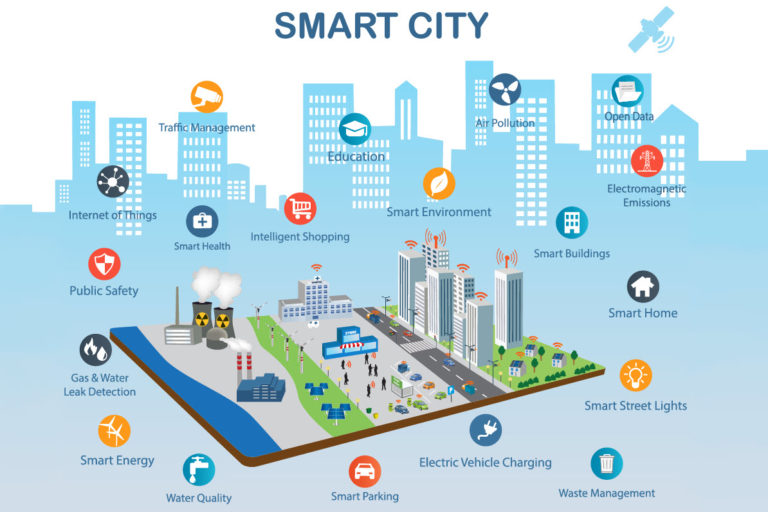
\includegraphics[width=0.5\textwidth]{images/smart-cities-infrastructure-iot-wide-768x512.jpg}
    \caption{Smart City Technologies \cite{b3}}
    \label{img:main_use_case}
\end{figure}
